\section{Điểm khác biệt so với giải pháp hiện có trên thị trường}

\subsection{Phân tích đối thủ cạnh tranh}

Qua khảo sát thị trường, Mutux chưa đối đầu trực tiếp với một nền tảng lớn chuyên cho \textbf{thuê thử gaming gear kết hợp Cọc Trả Sau}. Tuy nhiên, sản phẩm cạnh tranh gián tiếp với nhiều nhóm giải pháp đang giải quyết từng phần nhu cầu của người dùng.

\subsubsection{Showroom và chuỗi cửa hàng gaming gear}

\textbf{Đại diện}: GearVN, HACOM, Phong Vũ, XGear, GEARSHOP.

\begin{figure}[H]
    \centering
    
\includegraphics[width=0.7\textwidth]{PA2/img/gearvn.png}
    \caption{Showroom GearVN}
\end{figure}

Các cửa hàng này có lợi thế về thương hiệu, nguồn hàng mới, bảo hành chính hãng, tư vấn trực tiếp và khả năng mua ngay. Người dùng có thể đến showroom để xem sản phẩm, cầm thử một số mẫu chuột, bàn phím hoặc tai nghe trước khi mua.

\textbf{Điểm mạnh}
\begin{itemize}
    \item Có uy tín và độ tin cậy cao trên thị trường.
    \item Danh mục sản phẩm đa dạng, có nhiều thương hiệu lớn.
    \item Có bảo hành, hóa đơn và tư vấn trực tiếp.
    \item Phù hợp với người đã sẵn sàng mua sản phẩm.
\end{itemize}

\textbf{Điểm yếu}
\begin{itemize}
    \item Trải nghiệm thử tại showroom thường ngắn, không phản ánh cảm giác chơi game nhiều giờ.
    \item Không cho người dùng mang thiết bị về nhà để thử trong môi trường cá nhân.
    \item Không có cơ chế thuê thử độc lập trước khi mua.
    \item Dữ liệu đánh giá sau khi người dùng đã trải nghiệm thực tế nhiều ngày hạn chế.
\end{itemize}

\subsubsection{Gaming center và tiệm net cao cấp}

\textbf{Đại diện}: Vikings Gaming, CyberCore Gaming, G Gaming Center.

\begin{figure}[H]
    \centering
    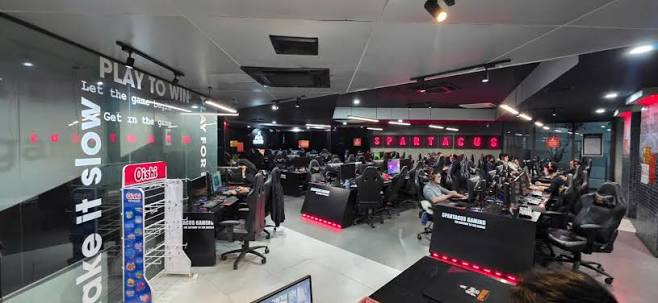
\includegraphics[width=0.6\textwidth]{PA2/img/ggear_2.jpg}
    \caption{G Gaming Center}
\end{figure}

Gaming center cho phép người chơi sử dụng chuột, bàn phím, tai nghe và màn hình trong môi trường chơi game thật. Đây là kênh trải nghiệm gần với nhu cầu thực tế hơn showroom vì người dùng có thể chơi game trực tiếp.

\textbf{Điểm mạnh}
\begin{itemize}
    \item Có môi trường chơi game thực tế.
    \item Chi phí trải nghiệm thấp theo giờ chơi.
    % \begin{figure}[H]
    % \centering
    % \includegraphics[width=0.86\textwidth]{img/ggaming.jpg}
    % \caption{Bảng giá dịch vụ của G Gaming Center}
% \end{figure}
    \item Có thể thử cảm giác sử dụng khi chơi game và kết hợp với các gear khác.
    \item Không cần giữ 1 số tiền lớn để cọc.
\end{itemize}

\textbf{Điểm yếu}
\begin{itemize}
    \item Người dùng chỉ trải nghiệm tại phòng máy, không thể mang thiết bị về nhà.
    \item Thiết bị thường dùng chung, hao mòn và không còn phản ánh đúng tình trạng sản phẩm mới.
    \item Số lượng mẫu gear giới hạn, phụ thuộc vào từng phòng máy, khó so sánh nhiều mẫu theo nhu cầu cá nhân.
    \item Không có hồ sơ chi tiết từng thiết bị, hầu như không có booking riêng cho từng món gear và không hỗ trợ mua sau khi thử.
\end{itemize}

% \subsubsection{Review online trên YouTube, TikTok và cộng đồng}

% \textbf{Đại diện}: YouTube, TikTok, Reddit, Facebook Group, các cộng đồng review gear gaming.

% Review online là nguồn tham khảo phổ biến vì người dùng có thể xem nhanh cảm nhận của reviewer, so sánh thông số, hình ảnh thực tế và ý kiến cộng đồng trước khi mua. Tuy nhiên, gaming gear là nhóm sản phẩm có tính cá nhân hóa cao: một con chuột hợp tay reviewer chưa chắc hợp với người dùng khác; một loại switch được nhiều người khen chưa chắc phù hợp với thói quen gõ hoặc chơi game riêng.

% \textbf{Điểm mạnh}
% \begin{itemize}
%     \item Dễ tiếp cận, chi phí gần như bằng không và có nhiều nội dung so sánh sản phẩm.
%     \item Giúp người dùng hiểu nhanh thông số, ưu nhược điểm và xu hướng cộng đồng.
%     \item Có thể tham khảo nhiều góc nhìn trước khi quyết định mua hoặc thuê thử.
% \end{itemize}

% \textbf{Điểm yếu}
% \begin{itemize}
%     \item Không thay thế được trải nghiệm thực tế theo form tay, lực gõ, độ thoải mái hoặc thói quen chơi game cá nhân.
%     \item Nhiều review chỉ phản ánh cảm nhận ngắn hạn, chưa chắc đúng với trải nghiệm sử dụng nhiều ngày.
%     \item Người dùng vẫn có rủi ro mua nhầm nếu chỉ dựa vào ý kiến của reviewer hoặc cộng đồng.
%     \item Review phân tán trên nhiều nền tảng, thiếu dữ liệu gắn trực tiếp với lịch sử thuê và trải nghiệm thật của từng thiết bị.
% \end{itemize}

\subsubsection{Website cho thuê thiết bị công nghệ}

\textbf{Đại diện}: \href{https://thuenhanh.vn/}{Thuê Nhanh}.

% \begin{figure}[H]
%     \centering
%     \includegraphics[width=0.86\textwidth]{img/thuenhanh.png}
%     \caption{Website Thuê Nhanh}
% \end{figure}
\begin{figure}[H]
    \centering
    \includegraphics[width=0.86\textwidth]{PA2/img/thuenhanh.png}
    \caption{Website Thuê Nhanh}
\end{figure}


Nhóm này đã có mô hình cho thuê tài sản công nghệ, giúp khách hàng thuê ngắn hạn thay vì mua mới. Danh mục thường tập trung vào laptop, PC, máy chơi game, màn hình hoặc thiết bị sự kiện, nên phù hợp với nhu cầu thuê thiết bị công nghệ nói chung.

\textbf{Điểm mạnh}
\begin{itemize}
    \item Người dùng có thể thuê thiết bị ngắn hạn thay vì phải mua mới.
    \item Có kinh nghiệm vận hành tài sản cho thuê, giao nhận và thu hồi thiết bị.
    \item Phù hợp với nhiều nhu cầu thuê: điện thoại, loa, xe máy/xe đạp, laptop, PC, console, màn hình hoặc thiết bị sự kiện.
\end{itemize}

\textbf{Điểm yếu}
\begin{itemize}
    \item Chưa đóng vai trò như một marketplace kết nối nhiều bên cho thuê với nhiều người thuê.
    \item Chưa tập trung vào thị trường gaming gear cá nhân như chuột, bàn phím cơ, tai nghe và tay cầm.
    \item Chưa có dữ liệu cộng đồng về đánh giá, số lượt thuê và mức độ hài lòng sau khi sử dụng.
    \item Chưa giải quyết rõ ràng rào cản tiền cọc bằng cơ chế Cọc Trả Sau.
    \item Chỉ hỗ trợ giao thiết bị ở Hà Nội và Thành phố Hồ Chí Minh.
\end{itemize}

\subsubsection{Shop bán gear hỗ trợ cho thuê gaming gear}

\textbf{Đại diện}: \href{https://quocdat.vn/}{Quốc Đạt Computer}, \href{https://ictsaigon.com.vn/?srsltid=AfmBOor5F5w1mZIggjDDyb7xtTYtj6N9P_WmJiGPTb4xZGrAjNpcsOCj}{ICT Sài Gòn}.

\begin{figure}[H]
    \centering
    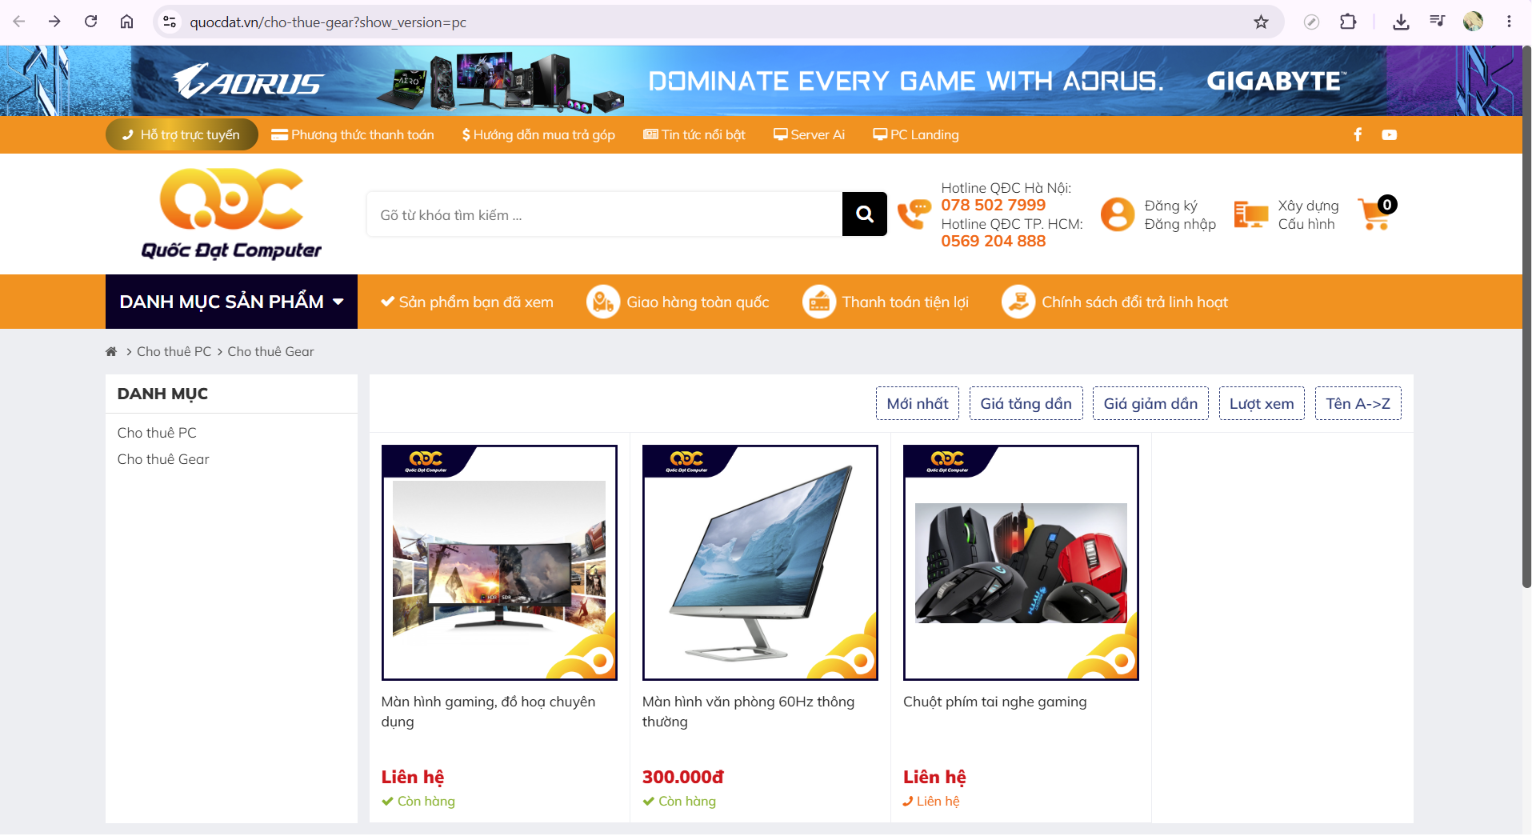
\includegraphics[width=0.86\textwidth]{PA2/img/quocdat.png}
    \caption{Website của Quốc Đạt Computer}
\end{figure}
\begin{figure}[H]
    \centering
    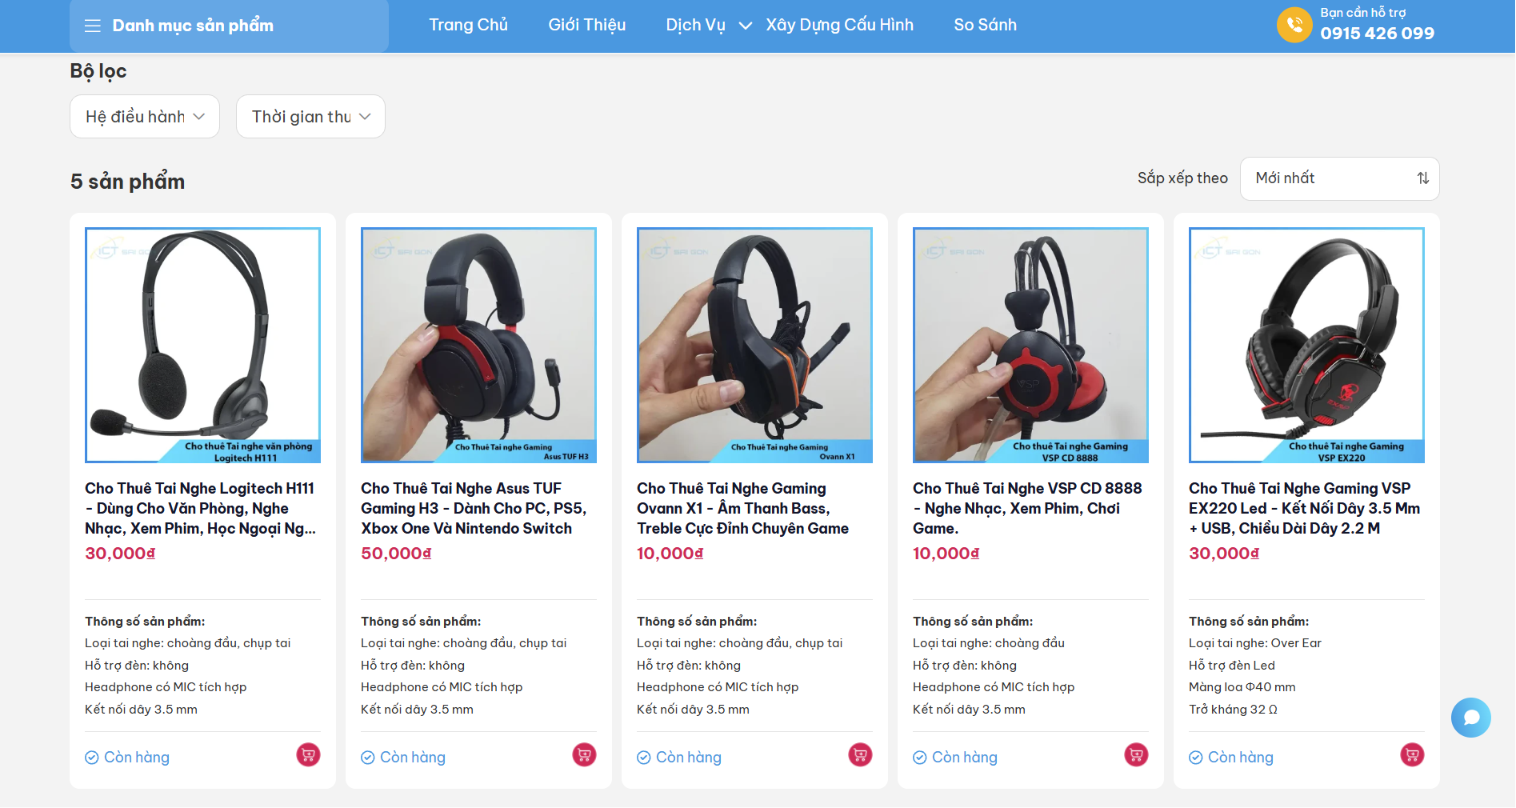
\includegraphics[width=0.86\textwidth]{PA2/img/ict.png}
    \caption{Website của ICT Sài Gòn}
\end{figure}

Nhóm này vốn có lợi thế về nguồn hàng gaming gear, hiểu sản phẩm và có tệp khách hàng đang quan tâm đến chuột, bàn phím, tai nghe, tay cầm hoặc phụ kiện gaming. Nếu mở rộng sang cho thuê, shop có thể tận dụng hàng trưng bày, hàng mẫu hoặc hàng tồn để tạo thêm doanh thu và giúp khách thử thiết bị trước khi mua.

\textbf{Điểm mạnh}
\begin{itemize}
    \item Có sẵn nguồn gear, kiến thức sản phẩm và khả năng tư vấn theo nhu cầu chơi game.
    \item Có thể kết hợp cho thuê thử với bán hàng để tăng tỷ lệ chuyển đổi mua sau trải nghiệm.
    \item Có thể tận dụng hàng mẫu, hàng trưng bày hoặc hàng tồn để tạo thêm doanh thu.
\end{itemize}

\textbf{Điểm yếu}
\begin{itemize}
    \item Chưa có hệ thống booking, quản lý lịch thuê và trạng thái từng thiết bị gear.
    \item Quy trình thuê còn thủ công, nhiều bước giấy tờ và chưa được số hóa hoàn toàn.
    \item Phạm vi giao nhận còn hạn chế, chưa hỗ trợ tốt người dùng ở các tỉnh xa thành phố lớn.
    \item Chưa tập trung vào thị trường gaming gear cá nhân hóa; danh mục cho thuê vẫn thiên về máy tính cấu hình cao.
    \item Chưa có dữ liệu công khai về đánh giá, số lượt thuê và lịch sử trải nghiệm của khách hàng.
    \item Chưa có Cọc Trả Sau để giảm rào cản tài chính cho người muốn thuê thử thiết bị giá trị cao.
\end{itemize}



\subsubsection{Marketplace và cộng đồng Facebook mua bán gaming gear}

\textbf{Đại diện}: \href{https://www.facebook.com/groups/919459388470044}{Chợ GearVN 2nd: Logitech-Zowie-Hyperx-Razer-Pulsar-Artisan-Glorious-Vaxee}, \href{https://www.facebook.com/groups/1140375019793944/about}{GEARVN - Chợ PC \& Gaming Gear}, các nhóm mua bán gear cũ trên Facebook.

\begin{figure}[H]
    \centering
    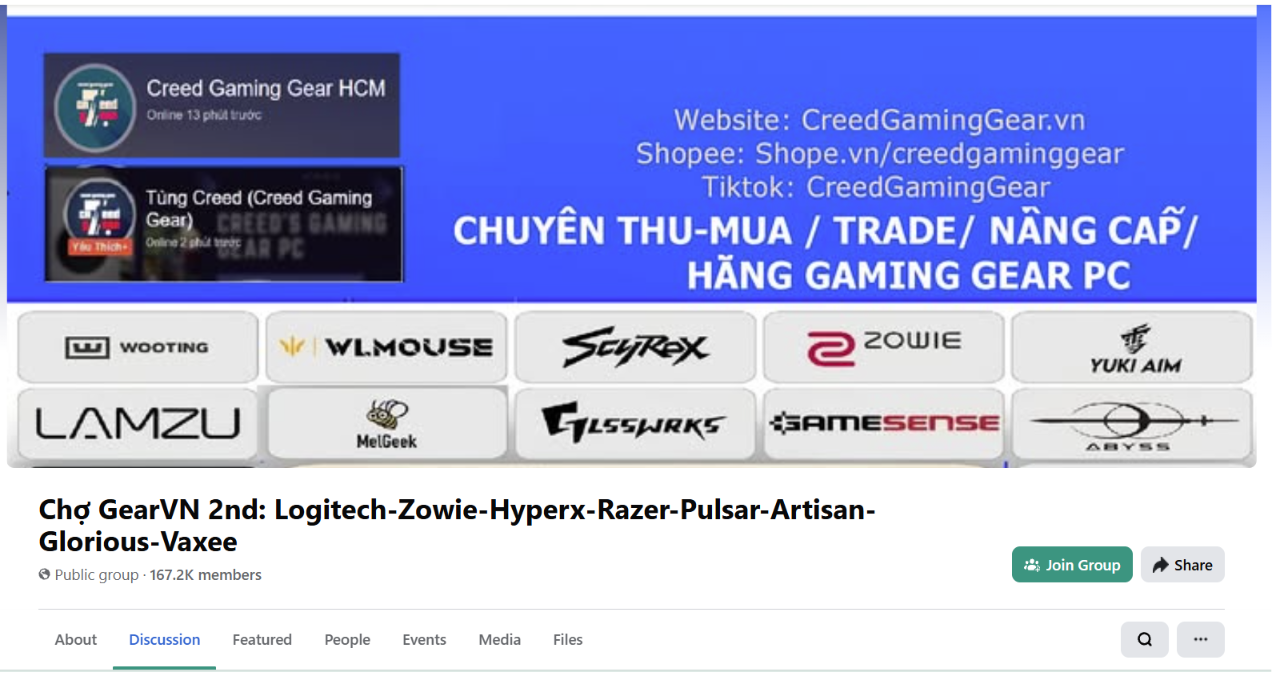
\includegraphics[width=0.86\textwidth]{PA2/img/fb_3.png}
    \caption{Group Chợ GearVN 2nd: Logitech-Zowie-Hyperx-Razer-Pulsar-Artisan-Glorious-Vaxee trên Facebook}
\end{figure}
\begin{figure}[H]
    \centering
    
\includegraphics[width=0.86\textwidth]{PA2/img/fb_2.png}
    \caption{Người đăng bài viết có nhu cầu thuê gear gaming trong nhóm}
\end{figure}

Nhóm này đáp ứng nhu cầu mua bán hoặc thuê mượn gaming gear giữa cá nhân với cá nhân. Người dùng có thể tìm được mức giá rẻ, sản phẩm hiếm, các mẫu đã ngừng bán hoặc thỏa thuận thuê thiết bị trực tiếp với người sở hữu gear.

\textbf{Điểm mạnh}
\begin{itemize}
    \item Giá mua hoặc thuê thường thấp.
    \item Nguồn cung lớn, có nhiều sản phẩm cũ, hiếm hoặc đã ngừng bán. Kết nối người thuê và người cho thuê ở mọi nơi.
    \item Giao dịch linh hoạt, người mua và người bán có thể tự thương lượng trực tiếp.
\end{itemize}

\textbf{Điểm yếu}
\begin{itemize}
    \item Khó xác thực tình trạng thật của thiết bị trước khi giao dịch.
    \item Dễ phát sinh rủi ro lừa đảo do giao dịch chủ yếu dựa trên niềm tin cá nhân.
    \item Không có hệ thống lưu bằng chứng giao nhận và lịch sử sử dụng.
    \item Không có bên trung gian xử lý tranh chấp hoặc cơ chế bảo chứng tài chính rõ ràng.
\end{itemize}
\subsubsection{Sàn thương mại điện tử và ứng dụng mua sắm}

\textbf{Đại diện}: \href{https://shopee.vn/}{Shopee}.

\begin{figure}[H]
    \centering
    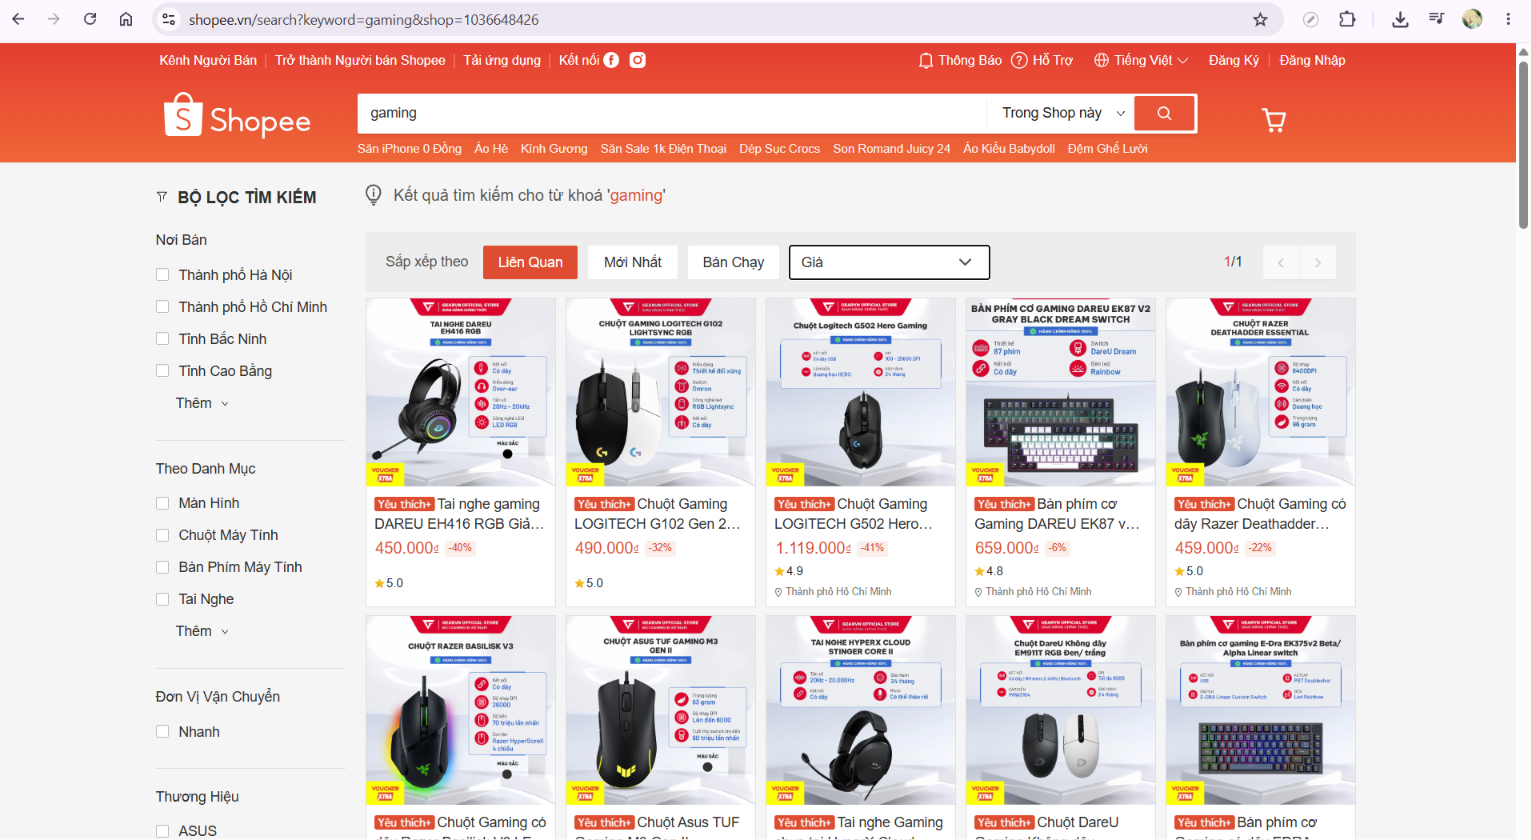
\includegraphics[width=0.86\textwidth]{PA2/img/shopee.png}
    \caption{Shopee}
\end{figure}

Một số sàn thương mại điện tử có chính sách đổi trả nếu không ưng ý, nhưng quá trình đổi trả thường phức tạp. Người dùng vẫn phải thanh toán toàn bộ giá trị sản phẩm trước, đồng thời có thể gặp rủi ro nếu sản phẩm đã qua sử dụng, thiếu phụ kiện, trầy xước hoặc không đáp ứng điều kiện đổi trả. Cách này phù hợp với người đã có ý định mua rõ ràng hơn là người chỉ muốn thử để so sánh.

\textbf{Điểm mạnh}
\begin{itemize}
    \item Nguồn cung rất lớn và dễ so sánh giá.
    \item Có hệ thống thanh toán, vận chuyển và khuyến mãi hoàn chỉnh.
    \item Có review sau mua và số lượng đơn bán.
    \item Phù hợp với người đã biết rõ sản phẩm muốn mua.
\end{itemize}

\textbf{Điểm yếu}
\begin{itemize}
    \item Người dùng không thể trải nghiệm thiết bị trước khi mua.
    \item Review thường đánh giá ngay sau khi mua, chưa chắc phản ánh trải nghiệm chơi game dài hạn.
    \item Việc đổi trả thường phức tạp, phụ thuộc vào chính sách từng sàn và từng shop.
    \item Người dùng vẫn phải thanh toán toàn bộ giá trị sản phẩm trước và có thể gặp rủi ro nếu sản phẩm đã qua sử dụng, thiếu phụ kiện, trầy xước hoặc không đáp ứng điều kiện đổi trả.
    \item Không có mô hình thuê thử, booking theo lịch hoặc chuyển phí thuê thành ưu đãi mua.
\end{itemize}




\subsection{So sánh Mutux với các giải pháp hiện có}
Các nhóm giải pháp hiện có đều giải quyết một phần nhu cầu nhưng chưa tạo thành một trải nghiệm liền mạch cho người muốn thử gaming gear trước khi mua. Showroom có sản phẩm mới nhưng chỉ cho thử nhanh; gaming center có môi trường chơi thật nhưng không cho mang thiết bị về nhà; website cho thuê có mô hình thuê nhưng chưa chuyên biệt cho gear; sàn thương mại điện tử mạnh về mua bán và chỉ phù hợp với người có ý định thực sự mua; cộng đồng Facebook có nguồn cung lớn nhưng thiếu xác thực và bảo chứng.

Từ đó, Mutux có thể nắm bắt các lỗ hổng sau:

\begin{itemize}
    \item Chưa có marketplace chuyên biệt cho thuê gaming gear cá nhân.
    \item Chưa có trải nghiệm thuê thử tại nhà trước khi quyết định mua.
    \item Chưa có booking theo lịch cho từng thiết bị gear.
    \item Chưa có review sau trải nghiệm thuê thực tế nhiều ngày.
    \item Chưa có quản lý bằng chứng giao nhận để giảm tranh chấp.
    \item Chưa có Cọc Trả Sau để giảm rào cản tài chính khi thuê thiết bị giá trị cao.
\end{itemize}

Bảng dưới đây tổng hợp các tiêu chí có thể dùng để so sánh Mutux với những giải pháp thay thế hiện có, bao gồm cả review trên TikTok, YouTube và các nền tảng/cộng đồng gear như một giải pháp tham khảo riêng. 



\begin{table}[H]
    \centering
    \footnotesize
    \renewcommand{\arraystretch}{1.28}
    \setlength{\tabcolsep}{4pt}
    \begin{tabular}{|p{4.4cm}|p{2.5cm}|p{2.5cm}|p{3.2cm}|p{2.2cm}|}
        \hline
        \textbf{Tiêu chí} & \textbf{Showroom gear} & \textbf{Gaming center} & \textbf{Review TikTok/YouTube, nền tảng chung} & \textbf{Mutux} \\
        \hline
        Tập trung riêng vào gaming gear cá nhân & Có & Một phần & Có nội dung chuyên biệt, nhưng không phải dịch vụ thuê & Có \\
        \hline
        Đa dạng chuột, bàn phím, tai nghe, tay cầm & Có & Hạn chế & Có, dưới dạng video/bài viết tham khảo & Có \\
        \hline
        Thuê gaming gear cá nhân ngắn hạn & Không & Không & Không & Có \\
        \hline
        Mang thiết bị về dùng tại nhà & Không & Không & Không & Có \\
        \hline
        Thử trước khi quyết định mua & Thử nhanh & Có tại chỗ & Không, chỉ xem cảm nhận từ reviewer/cộng đồng & Có \\
        \hline
        Booking theo lịch từng thiết bị & Không & Không & Không & Có \\
        \hline
        Lọc theo game, thông số và nhu cầu cá nhân & Một phần & Không & Phụ thuộc reviewer, thuật toán và cộng đồng & Có \\
        \hline
        Review sau trải nghiệm thuê nhiều ngày & Không & Không & Không, chủ yếu là review sau mua hoặc review ngắn hạn & Có \\
        \hline
        Hiển thị lượt thuê và lịch sử sử dụng & Không & Không & Không & Có \\
        \hline
        Quản lý bằng chứng giao nhận & Không & Không & Không & Có \\
        \hline
        Giải quyết tranh chấp qua nền tảng & Không & Không & Không & Có \\
        \hline
        Hỗ trợ cọc hoặc Cọc Trả Sau & Không & Không & Không & Có \\
        \hline
        Kết nối nhiều người thuê và cho thuê mọi nơi & Không & Không & Không & Có \\
        \hline
        Người cho thuê là shop và cá nhân độc lập & Không & Không & Không & Có \\
        \hline
        Tạo thêm doanh thu từ gear nhàn rỗi & Một phần & Không & Gián tiếp qua quảng bá & Có \\
        \hline
        Dữ liệu tập trung về cảm giác sử dụng gear & Không & Không & Có nhưng phân tán theo kênh, reviewer và nền tảng & Có \\
        \hline
    \end{tabular}
    \renewcommand{\arraystretch}{1}
    \caption{So sánh Mutux với showroom, gaming center và review online}
\end{table}

\begin{table}[H]
    \centering
    \footnotesize
    \renewcommand{\arraystretch}{1.28}
    \setlength{\tabcolsep}{4pt}
    \begin{tabular}{|p{4.4cm}|p{2.8cm}|p{2.8cm}|p{2.8cm}|p{2.2cm}|}
        \hline
        \textbf{Tiêu chí} & \textbf{Web thuê công nghệ} & \textbf{Sàn TMĐT} & \textbf{Group Facebook} & \textbf{Mutux} \\
        \hline
        Tập trung riêng vào gaming gear cá nhân & Không phổ biến & Có & Có & Có \\
        \hline
        Đa dạng chuột, bàn phím, tai nghe, tay cầm & Không phổ biến & Có & Có & Có \\
        \hline
        Thuê gaming gear cá nhân ngắn hạn & Một phần & Không & Có, tự phát & Có \\
        \hline
        Mang thiết bị về dùng tại nhà & Có & Có & Có nếu mua/thoả thuận & Có \\
        \hline
        Thử trước khi quyết định mua & Không rõ & Không & Không rõ & Có \\
        \hline
        Booking theo lịch từng thiết bị & Một phần & Không & Không & Có \\
        \hline
        Lọc theo game, thông số và nhu cầu cá nhân & Không phổ biến & Một phần & Không & Có \\
        \hline
        Review sau trải nghiệm thuê nhiều ngày & Không phổ biến & Một phần & Không hệ thống & Có \\
        \hline
        Hiển thị lượt thuê và lịch sử sử dụng & Không phổ biến & Không phải mô hình thuê & Không & Có \\
        \hline
        Quản lý bằng chứng giao nhận & Một phần & Có & Không & Có \\
        \hline
        Giải quyết tranh chấp qua nền tảng & Một phần & Một phần & Không & Có \\
        \hline
        Hỗ trợ cọc hoặc Cọc Trả Sau & Không & Không & Không & Có \\
        \hline
        Kết nối nhiều người thuê và cho thuê mọi nơi & Không & Không & Có, tự phát & Có \\
        \hline
        Người cho thuê là shop và cá nhân độc lập & Không phổ biến & Không & Có & Có \\
        \hline
        Tạo thêm doanh thu từ gear nhàn rỗi & Có & Không & Có, tự phát & Có \\
        \hline
        Dữ liệu tập trung về cảm giác sử dụng gear & Không phổ biến & Có nhưng thường là khoảng thời gian ngắn sau khi nhận hàng & Phân tán & Có \\
        \hline
    \end{tabular}
    \renewcommand{\arraystretch}{1}
    \caption{So sánh Mutux với web thuê công nghệ, sàn thương mại điện tử và group Facebook}
\end{table}

\subsection{Các điểm khác biệt chính của Mutux}

Lợi thế cạnh tranh của Mutux không nằm ở việc sở hữu một công nghệ quá khó sao chép, mà nằm ở khả năng chọn đúng thị trường ngách và giải quyết đúng nỗi đau của gamer. Trong khi phần lớn giải pháp hiện có tập trung vào bán sản phẩm, cung cấp review hoặc cho phép đổi trả sau khi mua, Mutux tập trung vào trải nghiệm \textbf{thử thật trước khi mua}, giúp người dùng giảm rủi ro mua nhầm thiết bị.

\subsubsection{Tập trung vào thị trường ngách gamer và eSports}

Mutux không phải là một nền tảng thuê đồ công nghệ chung chung, mà tập trung riêng vào chuột gaming, bàn phím cơ, tai nghe gaming, tay cầm và phụ kiện eSports. Đây là nhóm sản phẩm mà trải nghiệm cá nhân rất quan trọng, vì mỗi người có form tay, thói quen chơi game, cảm giác bấm và yêu cầu âm thanh khác nhau.

\subsubsection{Khác với shop bán gear truyền thống}

Các shop hiện tại chủ yếu bán sản phẩm, tư vấn, bảo hành hoặc thu cũ đổi mới. Người dùng vẫn phải ra quyết định mua trước khi có trải nghiệm đủ lâu với thiết bị. Mutux đảo ngược quá trình đó: người dùng được thuê thử trước, sau đó mới quyết định có nên mua hay không. Với shop, Mutux cũng tạo thêm một kênh khai thác thiết bị trưng bày, hàng mẫu hoặc sản phẩm chưa bán được bằng cách cho thuê ngắn hạn.

\subsubsection{Khác với dịch vụ thuê thiết bị gaming}

Một số đơn vị đã có dịch vụ thuê PC gaming, nhưng mục tiêu thường là cho thuê cả bộ máy phục vụ chơi game, livestream, sự kiện hoặc giải đấu. Mutux tập trung vào gear cá nhân, tức những thiết bị ảnh hưởng trực tiếp đến cảm giác chơi như chuột, bàn phím, tai nghe và tay cầm.

\subsubsection{Khác với mua online và chính sách đổi trả}

Mua online rồi đổi trả vẫn yêu cầu người dùng thanh toán toàn bộ giá trị sản phẩm trước và phụ thuộc vào điều kiện hoàn trả của từng shop hoặc sàn thương mại điện tử. Mutux tách nhu cầu trải nghiệm ra khỏi hành vi mua: người dùng chỉ thuê trong thời gian ngắn, trả chi phí thấp hơn và không phải giữ lại sản phẩm nếu cảm thấy không phù hợp. Điều này đặc biệt hữu ích với các sản phẩm có tính cá nhân cao như chuột gaming, bàn phím cơ và tai nghe.

\subsubsection{Mô hình hỗ trợ cọc giúp giảm rào cản thuê}

Ở các hình thức thuê truyền thống, tiền cọc thường là rào cản lớn vì người thuê phải khóa một khoản tiền gần bằng giá trị thiết bị. Mutux khác biệt ở việc cho phép người thuê chọn đặt cọc truyền thống hoặc sử dụng Cọc Trả Sau/hỗ trợ cọc. Khi đó, người dùng chỉ cần trả phí thuê và một khoản phí hỗ trợ nhỏ, trong khi bên cho thuê vẫn có cơ chế bảo chứng để xử lý rủi ro mất mát hoặc hư hỏng thiết bị.

\subsubsection{Tạo dữ liệu review thực tế sau khi thuê}

Review trên mạng thường mang tính chung chung hoặc đến từ reviewer chuyên nghiệp. Mutux có thể thu thập đánh giá từ người dùng thật sau khi họ đã thuê thiết bị và chơi game trong bối cảnh thực tế. Ví dụ, người dùng có thể đánh giá chuột có hợp tay không, tai nghe có đau tai sau ba giờ sử dụng không, switch có gây mỏi tay không, hoặc tay cầm có bị delay khi chơi FC Online không.

Đây là loại dữ liệu có giá trị vì gắn trực tiếp với trải nghiệm sử dụng thật. Nếu đối thủ mới tham gia thị trường, họ khó có ngay lượng dữ liệu hành vi và review thực tế tương tự.

\subsubsection{Có thể tạo mạng lưới hai phía}

Mutux có thể phát triển thành mạng lưới hai phía: một bên là gamer muốn thuê hoặc thử gear, bên còn lại là shop hoặc cá nhân có gear muốn cho thuê để kiếm thêm thu nhập. Khi càng nhiều thiết bị được đăng lên, người dùng càng có nhiều lựa chọn. Khi càng nhiều người dùng thuê, shop và chủ gear càng có động lực đưa thêm thiết bị lên nền tảng.

Nếu triển khai tốt, hiệu ứng mạng lưới này sẽ trở thành một lợi thế cạnh tranh quan trọng, vì giá trị của nền tảng tăng lên cùng với số lượng người dùng và số lượng thiết bị đang lưu thông trên hệ thống.

Tóm lại, Mutux khác biệt vì kết hợp năm yếu tố trong cùng một nền tảng: \textbf{marketplace chuyên cho thuê gaming gear}, \textbf{trải nghiệm thử thật trước khi mua}, \textbf{review sau trải nghiệm thực tế}, \textbf{Cọc Trả Sau/hỗ trợ cọc} và \textbf{mạng lưới hai phía giữa người thuê với shop/chủ gear}. Sự kết hợp này giúp Mutux khác với shop bán gear, review online, mua online đổi trả, mua gear cũ và các dịch vụ thuê thiết bị công nghệ chung chung.

